\documentclass[tikz,border=1mm]{standalone}

\usepackage{amsmath}
\usepackage{graphicx}
\renewcommand\familydefault{\sfdefault} 
\usepackage[T1]{fontenc}

\usetikzlibrary{arrows,shapes,calc}
\tikzset{every picture/.style={/utils/exec={\sffamily}}}

\begin{document}

% Radian
% \begin{tikzpicture}
%     \draw [thick,blue] circle (2);
%     \draw [thick] (0, 0) -- (0:2) arc (0:{180/pi}:2) -- (0, 0);
%     \draw [-latex'] (0:0.5) arc (0:{180/pi}:0.5);
%     \node at ({90/pi}:0.5) [anchor=south west] {$1 \,\text{rad}$};
%     \draw [latex'-latex'] (270:0.2) -- ++(0:2) node [below,pos=0.5] {$r$};
%     \draw [latex'-latex'] ({180/pi+90}:0.2) -- ++({180/pi}:2) node [above,pos=0.5,rotate={180/pi}] {$r$};
%     \draw [latex'-latex'] (0:2.2) arc (0:{180/pi}:2.2) node [right,pos=0.5] {$r$};
% \end{tikzpicture}

% % Triangle
% \begin{tikzpicture}
%     \draw [thick] (0, 0) node [left] {$A$} 
%         -- node [below] {$\text{adjacent}$} ++(4, 0) node [right] {$B$} 
%         -- node [above,rotate=-90] {$\text{opposite}$} ++(0, 3) node [right] {$C$} 
%         -- node [above,rotate={atan(3/4)}] {$\text{hypotenuse}$} (0, 0);
%     \draw (3.8, 0) -- ++(0, 0.2) -- ++(0.2, 0);
%     \draw (0:1) arc (0:{atan(3/4)}:1);
%     \node at ({atan(3/4)/2}:0.67) {$\theta$};
% \end{tikzpicture}

% % Circle
% \begin{tikzpicture}
%     \draw [-stealth'] (-1, 0) -- (4, 0) node [below] {$x$};
%     \draw [-stealth'] (0, -1) -- (0, 4) node [left] {$y$};
%     \draw [blue,thick] (-20:3) arc (-20:110:3);
%     \draw [fill] (45:3) circle (2pt) node [above right] {$(x, y)$};
%     \draw (0, 0) -- ++({3 * cos(45)}, 0) -- ++(0, {3 * sin(45)}) -- node [above,rotate=45] {$r$} (0, 0);
%     \draw ({3 * cos(45) - 0.2}, 0) -- ++(0, 0.2) -- ++(0.2, 0);
%     \draw [-latex'] (1, 0) arc (0:45:1);
%     \node at (22.5:0.67) {$\theta$};
%     \draw [latex'-latex'] (0, -0.2) -- ++({3 * cos(45)}, 0) node [below, pos=0.5] {$r\cos(\theta)$};
%     \draw [latex'-latex'] ({3 * cos(45) + 0.2}, 0) -- ++(0, {3 * sin(45)}) node [right, pos=0.5] {$r\sin(\theta)$};
% \end{tikzpicture}

% Sine wave
% \begin{tikzpicture}
%     \draw [-stealth'] (-2.5, 0) -- (2.5, 0) node [below] {$x$};
%     \draw [-stealth'] (0, -2.5) -- (0, 2.5) node [left] {$y$};
%     \draw [blue,thick] circle (2);
%     \draw [latex'-latex'] (0, 0) -- (135:2) node [pos=0.5,above,rotate=-45] {$r=1$};
%     \draw (0, 0) -- (45:2);
%     \draw [-latex'] (0:1) arc (0:45:1);
%     \draw [fill] (45:2) circle (2pt);
%     \node at (22.5:0.67) {$\frac{\pi}{4}$};
%     \draw [-stealth'] (4, 0) -- ++(11, 0) node [below] {$\theta$};
%     \draw [-stealth'] (4, -2.5) -- (4, 2.5) node [left] {$y$};
%     \node [below] at ({4 + 45/36}, 0) {$\frac{\pi}{2}$};
%     \node [below] at ({4 + 90/36}, 0) {$\pi$};
%     \node [below] at ({4 + 135/36}, 0) {$\frac{3\pi}{2}$};
%     \node [below] at ({4 + 180/36}, 0) {$2\pi$};
%     \node [below] at ({4 + 225/36}, 0) {$\frac{5\pi}{2}$};
%     \node [below] at ({4 + 270/36}, 0) {$3\pi$};
%     \node [below] at ({4 + 315/36}, 0) {$\frac{7\pi}{2}$};
%     \node [below] at ({4 + 360/36}, 0) {$4\pi$};
%     \node [left] at (4, -2) {$-1$};
%     \node [left] at (4, 2) {$1$};
%     \draw [domain=0:720,samples=200,blue,thick] plot ({4+\x/72}, {2 * sin(\x)});
%     \draw [fill] ({4 + 45/72}, {2 * sin(45)}) circle (2pt);
%     \draw [fill] ({4 + 405/72}, {2 * sin(405)}) coordinate (1) circle (2pt);
%     \draw [dashed] (45:2) -- (1);
% \end{tikzpicture}

% % Amplitude
% \begin{tikzpicture}
%     \draw [-stealth'] (0, 0) -- ++(11, 0) node [below] {$\theta$};
%     \draw [-stealth'] (0, -2.5) -- (0, 2.5) node [left] {$y$};
%     \node [below] at ({180/72}, 0) {$\pi$};
%     \node [below] at ({360/72}, 0) {$2\pi$};
%     \node [below] at ({540/72}, 0) {$3\pi$};
%     \node [below] at ({720/72}, 0) {$4\pi$};
%     \draw [domain=0:740,samples=200,blue,thick] plot ({\x/72}, {sin(\x)}) node [right] {$y = \sin(\theta)$};
%     \draw [domain=0:740,samples=200,red,thick] plot ({\x/72}, {2 * sin(\x)}) node [above right] {$y = A\sin(\theta)$};
%     \draw [latex'-latex'] ({445/72}, 0) -- ++(0, {2*sin{90}}) node [right,pos=0.67] {$A$};
%     \draw [latex'-latex'] ({455/72}, 0) -- ++(0, {sin{90}}) node [right,pos=0.5] {$1$};
%     \draw [latex'-latex'] ({265/72}, 0) -- ++(0, {2*sin{270}}) node [right,pos=0.67] {$A$};
%     \draw [latex'-latex'] ({275/72}, 0) -- ++(0, {sin{270}}) node [right,pos=0.5] {$1$};
% \end{tikzpicture}

% % Frequency
% \begin{tikzpicture}
%     \draw [-stealth'] (0, 0) -- ++(11, 0) node [below] {$\theta$};
%     \draw [-stealth'] (0, -2.5) -- (0, 2.5) node [left] {$y$};
%     \node [below] at ({180/72}, 0) {$\pi$};
%     \node [below] at ({360/72}, 0) {$2\pi$};
%     \node [below] at ({540/72}, 0) {$3\pi$};
%     \node [below] at ({720/72}, 0) {$4\pi$};
%     \node [left] at (0, -2) {$-1$};
%     \node [left] at (0, 2) {$1$};
%     \draw [domain=0:740,samples=200,blue,thick] plot ({\x/72}, {2 * sin(\x)}) node [right] {$y = \sin(\theta)$};
%     \draw [domain=0:740,samples=200,red,thick] plot ({\x/72}, {2 * sin(2 * \x)}) node [right] {$y = \sin(2\theta)$};
% \end{tikzpicture}

% % Phase
% \begin{tikzpicture}
%     \draw [-stealth'] (0, 0) -- ++(11, 0) node [below] {$\theta$};
%     \draw [-stealth'] (0, -2.5) -- (0, 2.5) node [left] {$y$};
%     \node [below] at ({90/72}, 0) {$\frac{\pi}{2}$};
%     \node [below] at ({180/72}, 0) {$\pi$};
%     \node [below] at ({270/72}, 0) {$\frac{3\pi}{2}$};
%     \node [below] at ({360/72}, 0) {$2\pi$};
%     \node [below] at ({450/72}, 0) {$\frac{5\pi}{2}$};
%     \node [below] at ({540/72}, 0) {$3\pi$};
%     \node [below] at ({630/72}, 0) {$\frac{7\pi}{2}$};
%     \node [below] at ({720/72}, 0) {$4\pi$};
%     \node [left] at (0, -2) {$-1$};
%     \node [left] at (0, 2) {$1$};
%     \draw [domain=0:740,samples=200,blue,thick] plot ({\x/72}, {2 * sin(\x)}) node [right] {$y = \sin(\theta)$};
%     \draw [domain=0:740,samples=200,red,thick] plot ({\x/72}, {2 * sin(\x + 45)}) node [right] {$y = \sin(\theta + \phi)$};
%     \draw [-latex'] ({380/72}, {2 * sin(380)}) -- ++(-{45/72}, 0) node [above,pos=0.33] {$\phi$};
% \end{tikzpicture}


% Sum of sines
% \begin{tikzpicture}
%     \draw [-stealth'] (0, 0) -- ++(11, 0) node [below] {$\theta$};
%     \draw [-stealth'] (0, -2.5) -- (0, 8) node [left] {$y$};
%     \node [below] at ({90/72}, 0) {$\frac{\pi}{2}$};
%     \node [below] at ({180/72}, 0) {$\pi$};
%     \node [below] at ({270/72}, 0) {$\frac{3\pi}{2}$};
%     \node [below] at ({360/72}, 0) {$2\pi$};
%     \node [below] at ({450/72}, 0) {$\frac{5\pi}{2}$};
%     \node [below] at ({540/72}, 0) {$3\pi$};
%     \node [below] at ({630/72}, 0) {$\frac{7\pi}{2}$};
%     \node [below] at ({720/72}, 0) {$4\pi$};
%     \draw [domain=0:740,samples=200,blue,thick] plot ({\x/72}, {4.5+2/5+2/3+1+sin(\x)}) node [right] {$y = 2\sin(\theta)$};
%     \draw [domain=0:740,samples=200,blue,thick] plot ({\x/72}, {3.5+2/5+2/3+2/3*sin(3*\x)}) node [right] {$y = \dfrac{2}{3}\sin(3\theta)$};
%     \draw [domain=0:740,samples=200,blue,thick] plot ({\x/72}, {2.5+2/5+2/5*sin(5*\x)}) node [right] {$y = \dfrac{2}{5}\sin(5\theta)$};
%     % \draw [domain=0:740,samples=200,blue,thick] plot ({\x/72}, {3+2/7*sin(7*\x)}) node [right] {$y = \dfrac{2}{7}\sin(7\theta)$};
%     \draw [domain=0:740,samples=200,red,thick] plot ({\x/72}, {2*sin(\x) + 2/3*sin(3*\x) + 2/5*sin(5*\x)}) node [right] {sum of sines};
% \end{tikzpicture}


% % Flow chart
% \tikzstyle{block} = [rectangle, minimum width=2cm, text width=2.75cm, minimum height=1cm,text centered,node distance=2.5cm,anchor=north]
% \tikzstyle{arrow} = [ultra thick,->,>=stealth]
% \begin{tikzpicture}[node distance=5cm]
%     \node (performance) {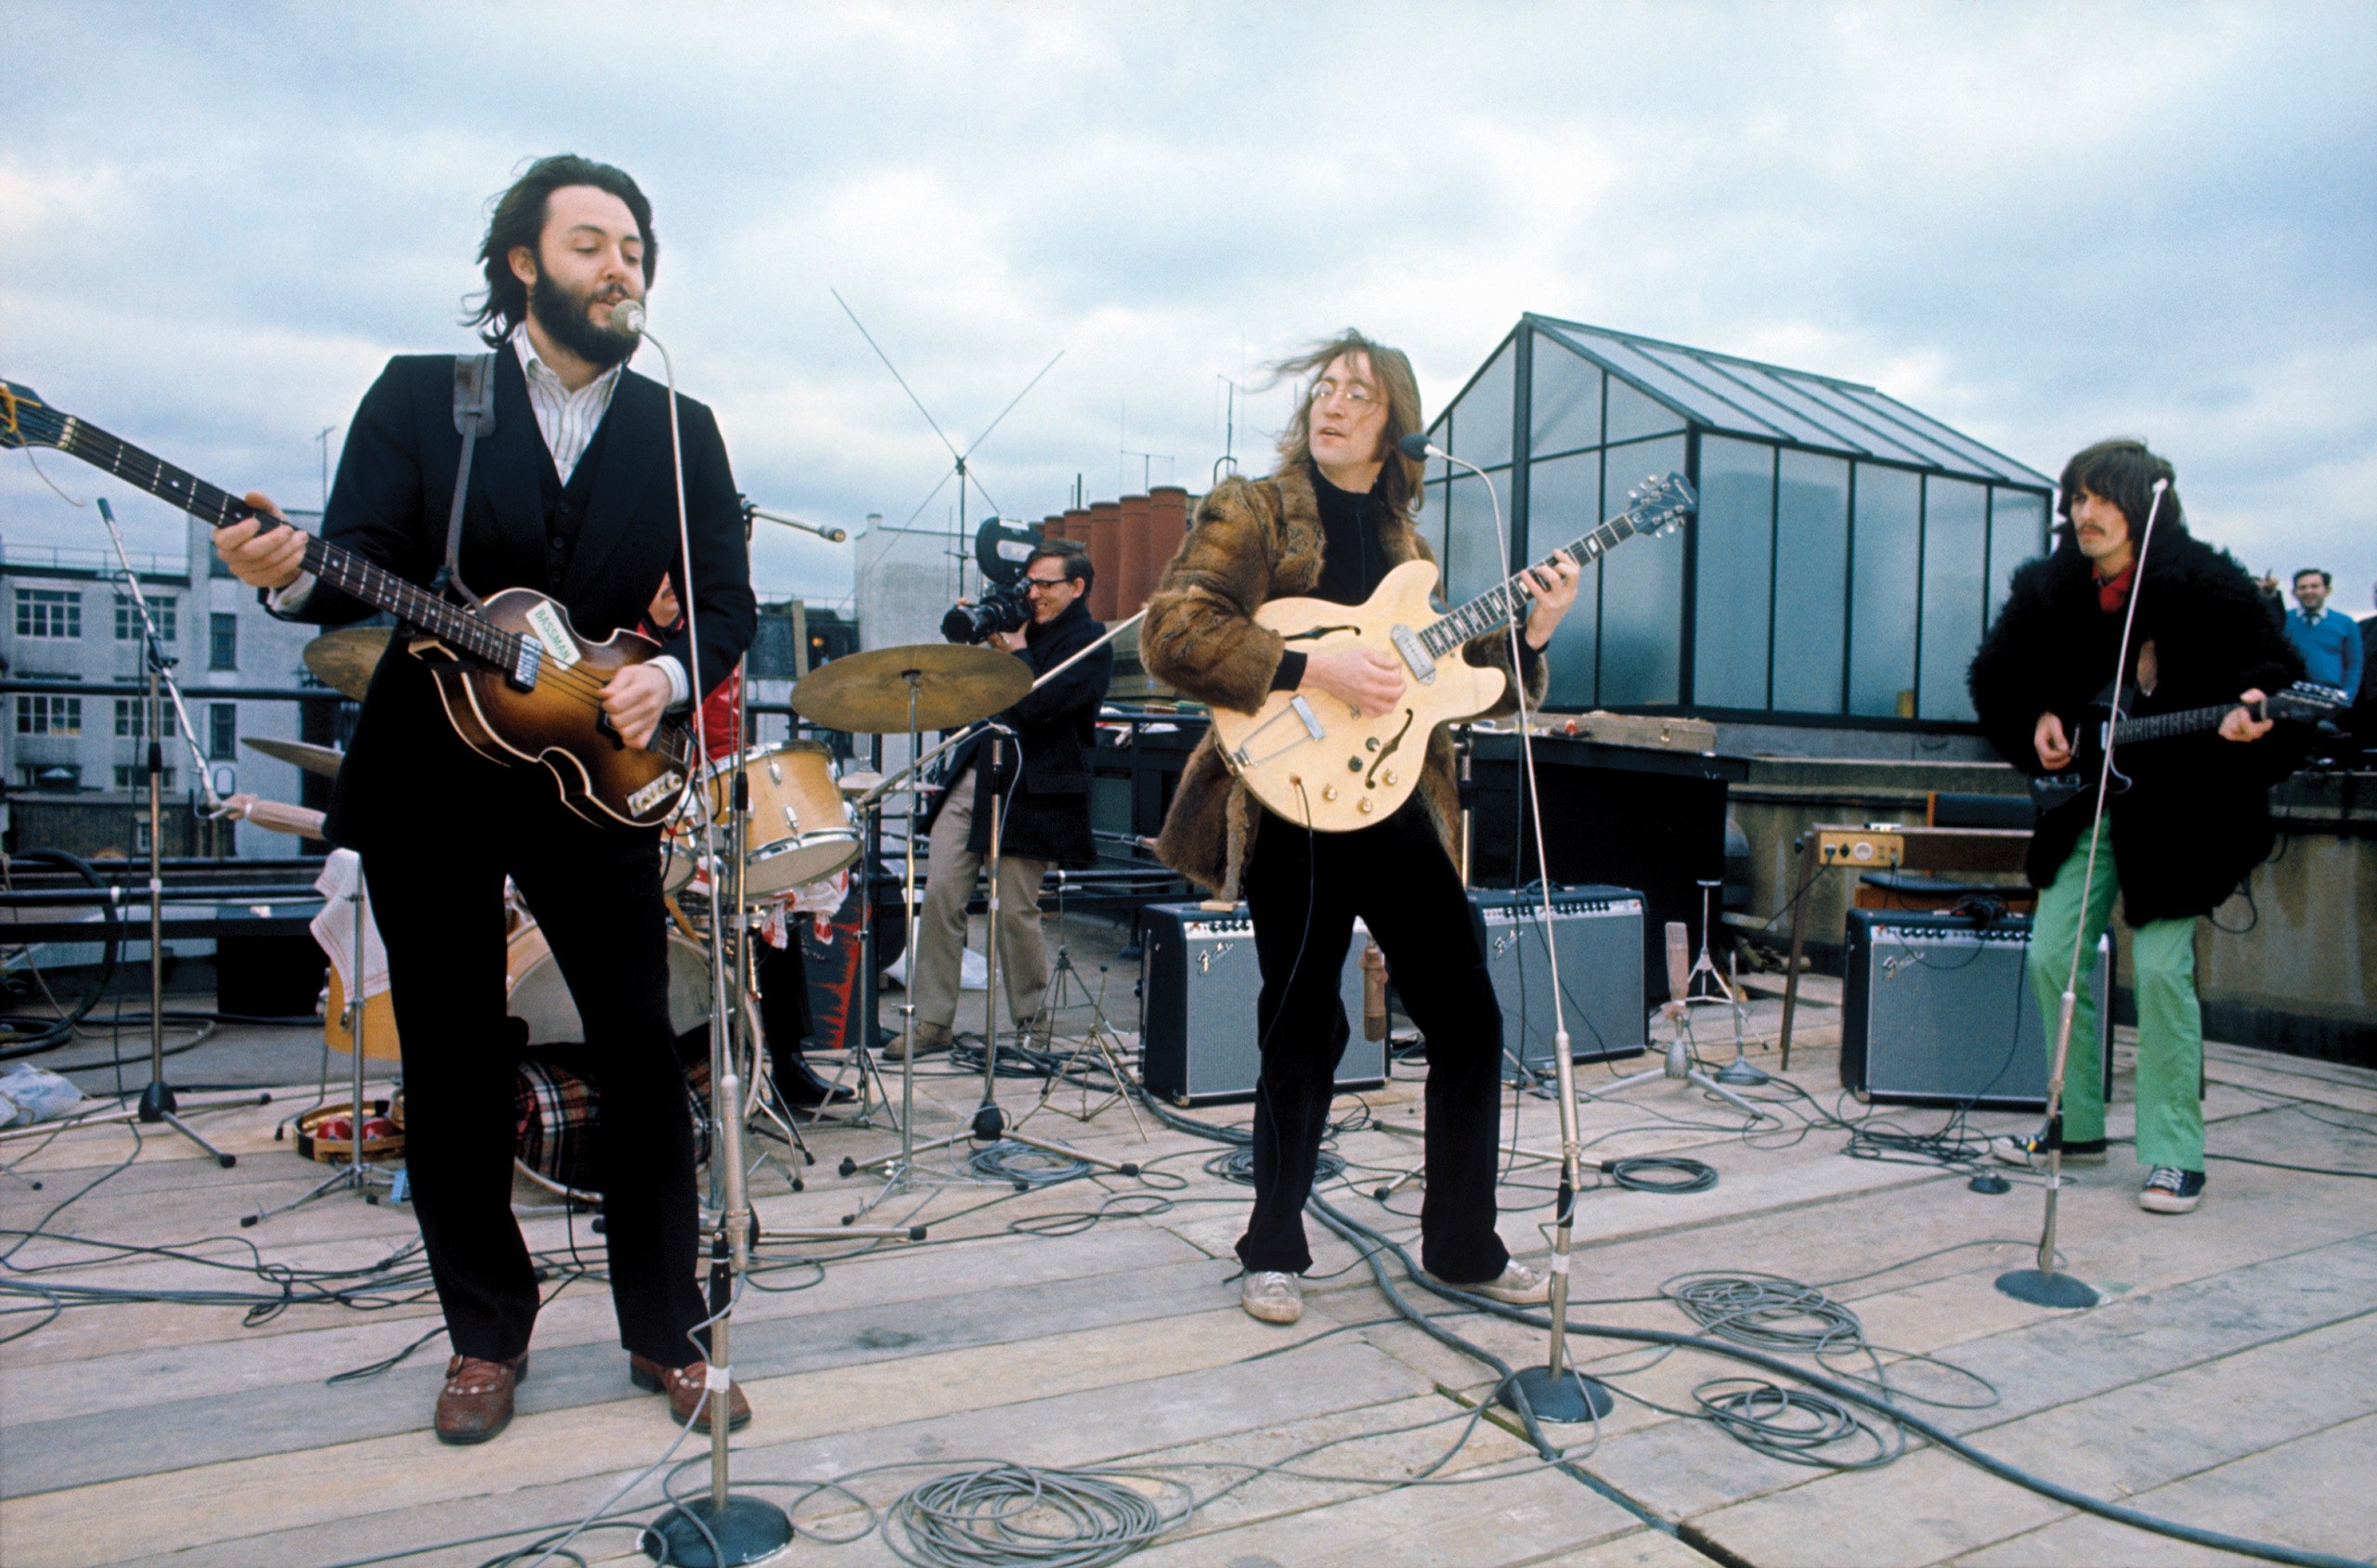
\includegraphics[width=5cm]{./beatles.jpeg}};
%     \node [right of=performance,node distance=5.5cm] (digital) {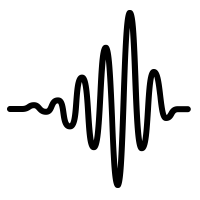
\includegraphics[width=3cm]{sound_wave.jpeg}};
%     \node [right of=digital] (fourier) {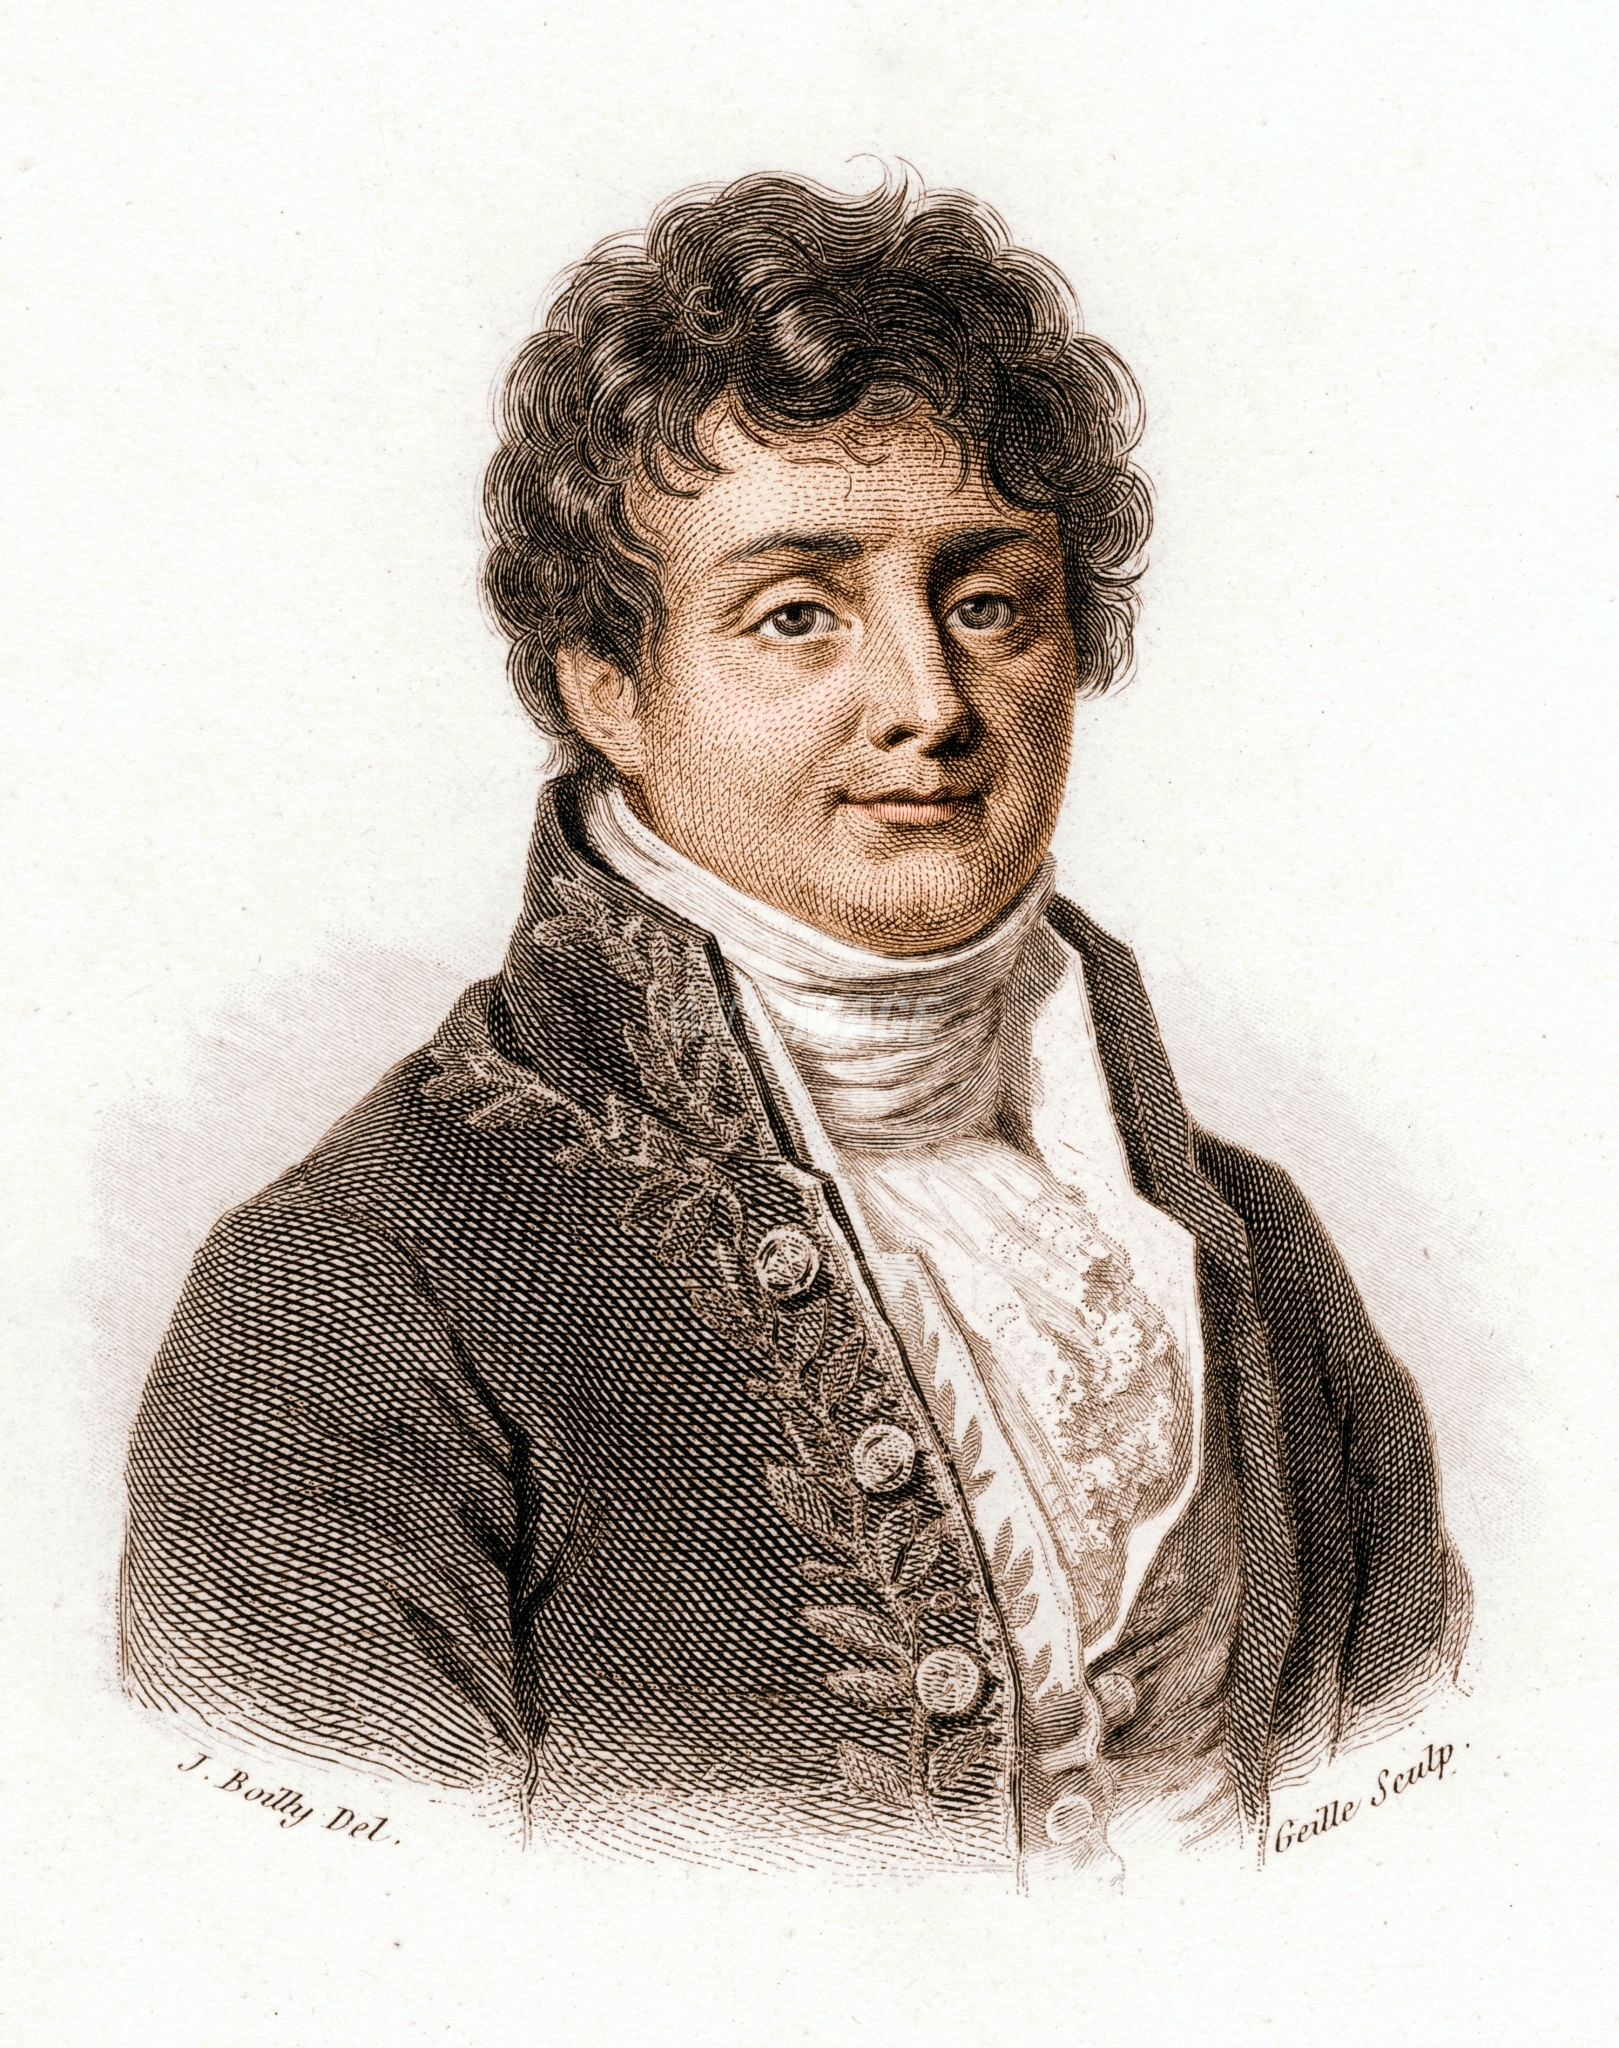
\includegraphics[width=3cm]{Fourier.jpeg}};
%     \node [right of=fourier] (discard) {
\includegraphics[width=3cm]{discard.png}};
%     \node [below of=discard] (inverse fourier) {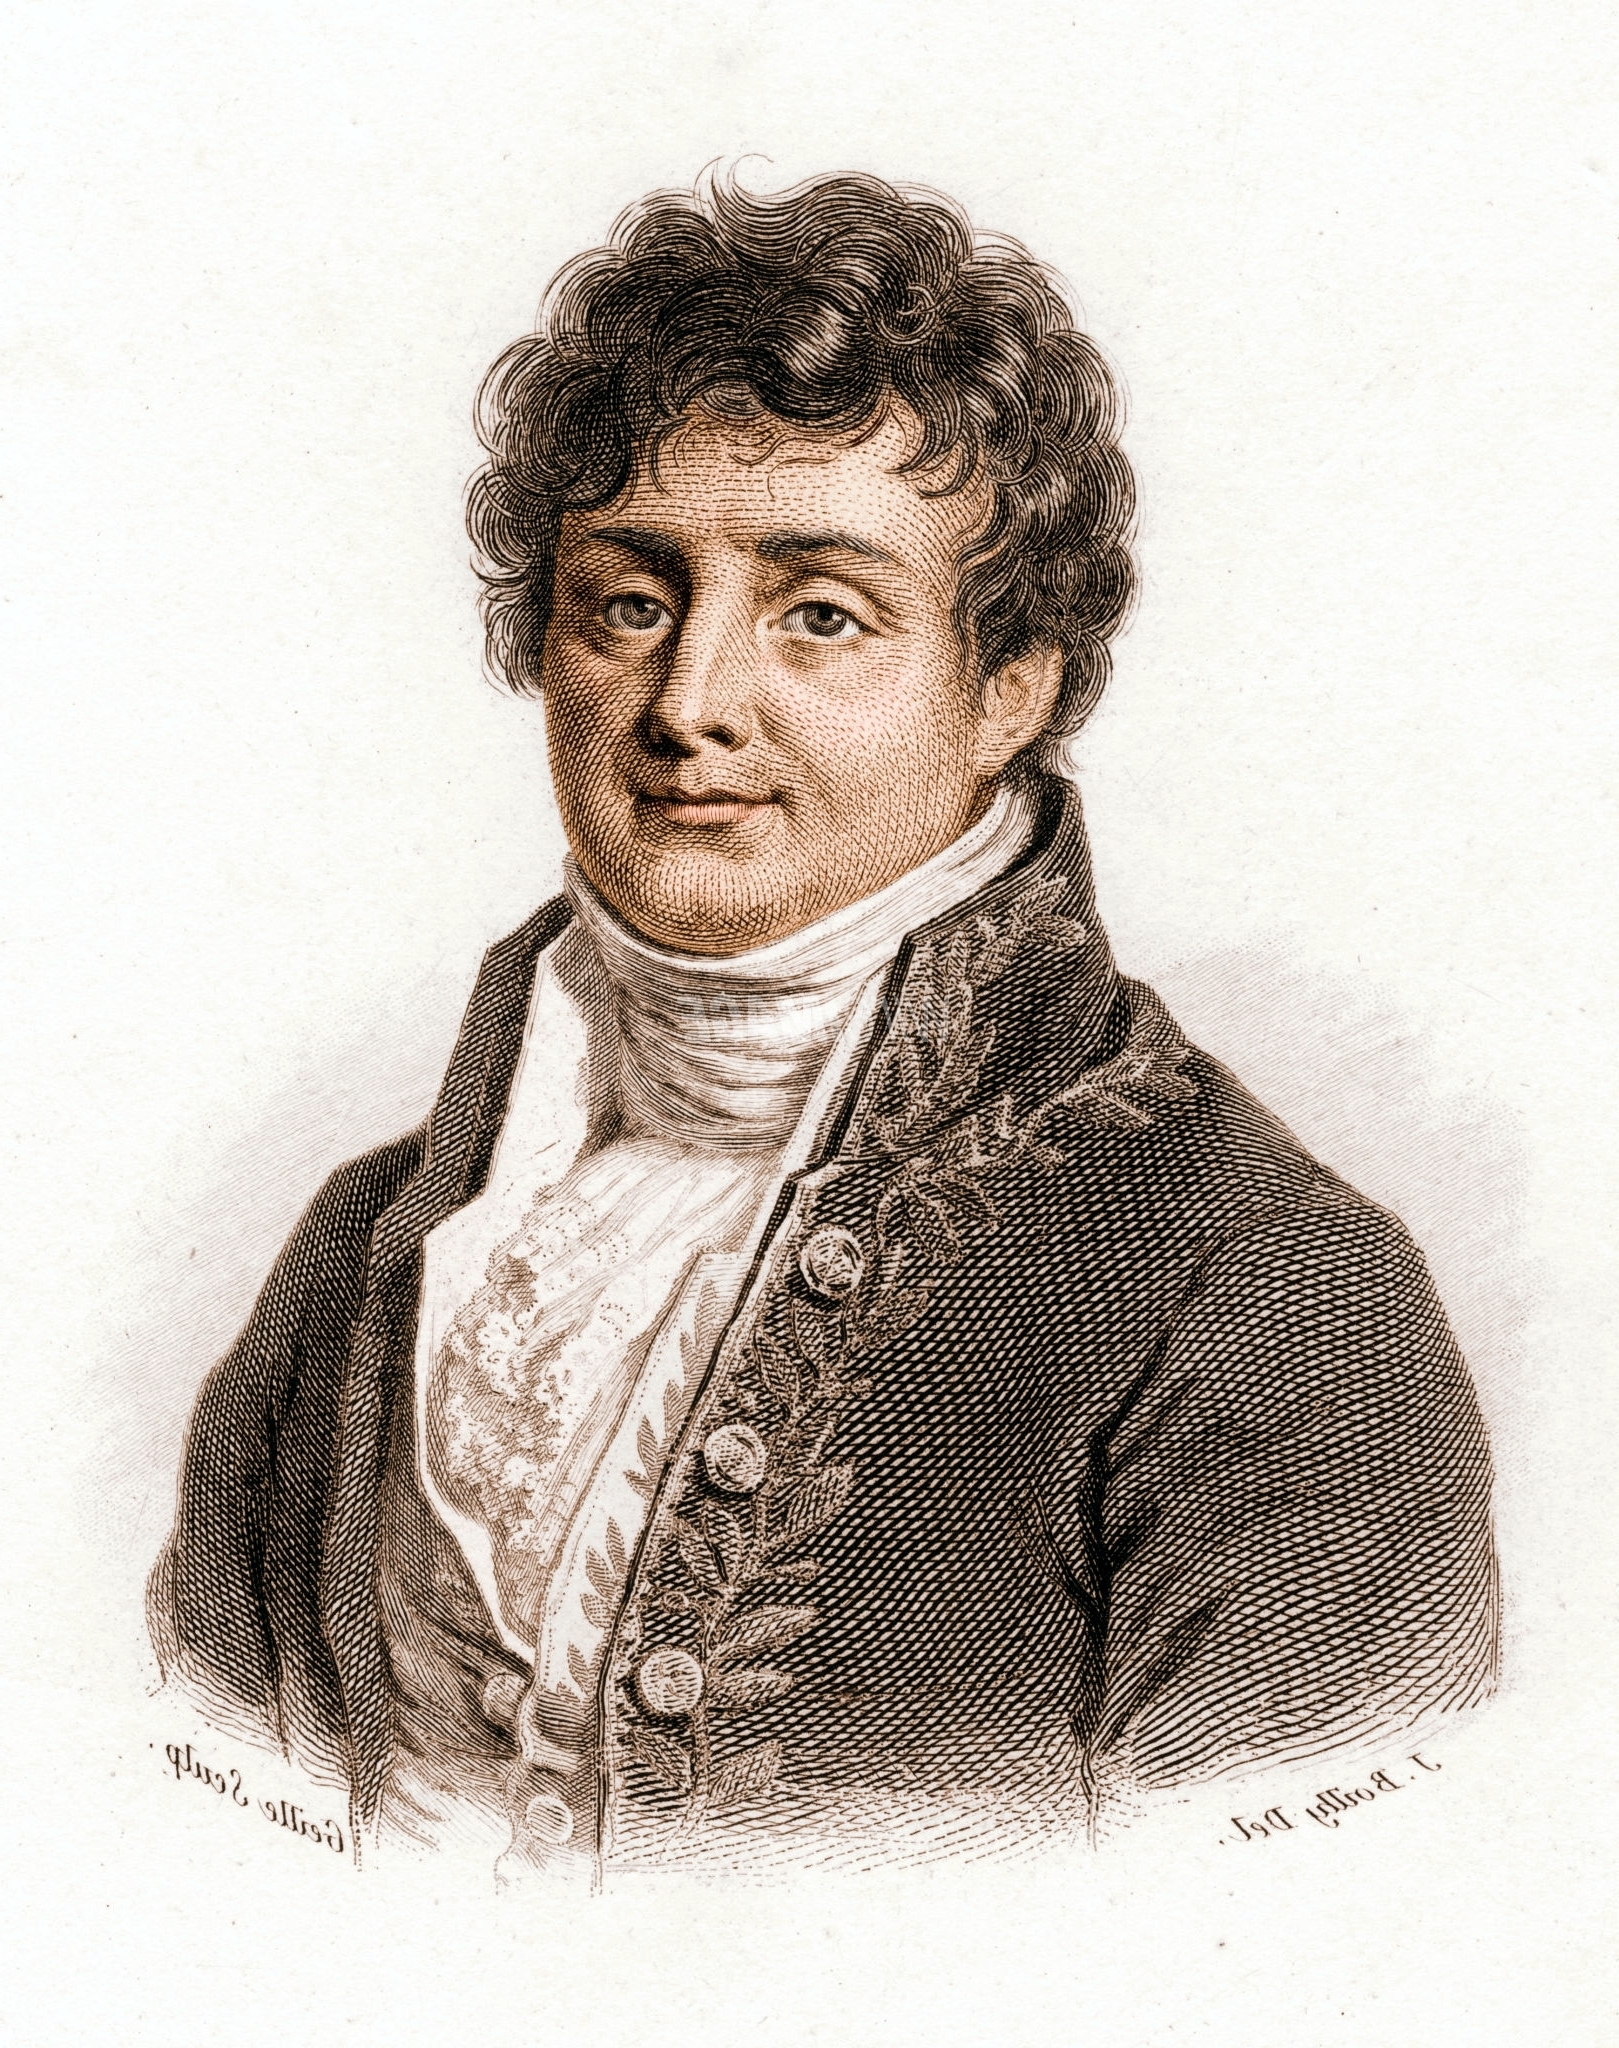
\includegraphics[width=3cm]{Inverse Fourier.jpeg}};
%     \node [left of=inverse fourier] (reconstruct) {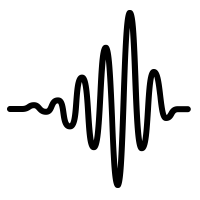
\includegraphics[width=3cm]{sound_wave.jpeg}};
%     \node [left of=reconstruct] (stream) {
\includegraphics[width=3cm]{spotify.png}};
%     \node [left of=stream] (play) {
\includegraphics[width=3cm]{listen.jpeg}};
%     \draw [arrow] (performance) -- (digital);
%     \draw [arrow] (digital) -- (fourier);
%     \draw [arrow] (fourier) -- (discard);
%     \draw [arrow] (discard) -- (inverse fourier);
%     \draw [arrow] (inverse fourier) -- (reconstruct);
%     \draw [arrow] (reconstruct) -- (stream);
%     \draw [arrow] (stream) -- (play);
%     \node [block,above of=performance] {Record music};
%     \node [block,above of=digital] {Sound signal};
%     \node [block,above of=fourier] {Calculate Fourier transform};
%     \node [block,above of=discard] {Discard inaudible frequencies};
%     \node [block,below of=inverse fourier] {Calculate inverse Fourier transform};
%     \node [block,below of=reconstruct] {Reconstruct sound signal};
%     \node [block,below of=stream] {Stream over the internet};
%     \node [block,below of=play] {Listen};
% \end{tikzpicture}

% Piano
% \begin{tikzpicture}
%     \foreach \i in {0, ..., 51}{
%         \draw (\i * 0.4, 0) rectangle ++(0.4, 2);
%     }
%     \draw [fill] (0.3, 0.75) rectangle ++(0.2, 1.25);
%     \foreach \i in {0, ..., 6}{
%         \draw [fill] (1.1 + 2.8 * \i, 0.75) rectangle ++(0.2, 1.25);
%         \draw [fill] (1.5 + 2.8 * \i, 0.75) rectangle ++(0.2, 1.25);
%     }
%     \foreach \i in {0, ..., 6}{
%         \draw [fill] (2.3 + 2.8 * \i, 0.75) rectangle ++(0.2, 1.25);
%         \draw [fill] (2.7 + 2.8 * \i, 0.75) rectangle ++(0.2, 1.25);
%         \draw [fill] (3.1 + 2.8 * \i, 0.75) rectangle ++(0.2, 1.25);
%     }
%     \node (A4) at (11.4, -1) {A4};
%     \draw [-latex'] (A4) -- ++(0, 1);
%     \node [align=center] (A4) at (9.4, -1) {C4 \\ ``middle C''};
%     \draw [-latex'] (A4) -- ++(0, 1);
% \end{tikzpicture}

% Piano A chord
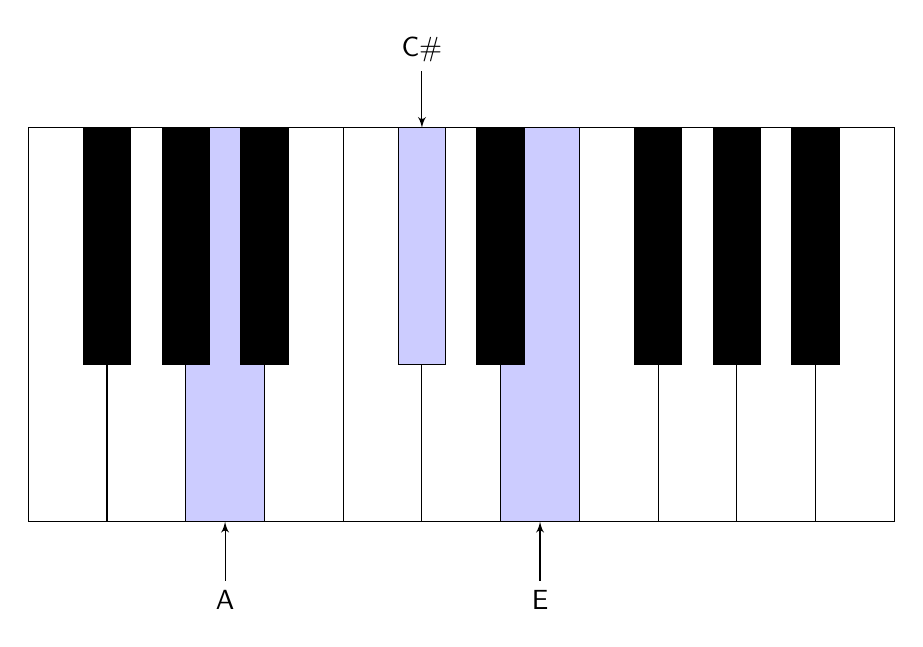
\begin{tikzpicture}
    \fill [blue!20] (2, 0) rectangle ++(1, 5);
    \fill [blue!20] (6, 0) rectangle ++(1, 5);
    \foreach \i in {0, ..., 10}{
        \draw (\i, 0) rectangle ++(1, 5);
    }
    \foreach \i in {0, 1}{
        \draw [fill] (4.7 + \i, 2) rectangle ++(0.6, 3);
    }
    \foreach \i in {0, ..., 2}{
        \draw [fill] (0.7 + \i, 2) rectangle ++(0.6, 3);
    }
    \foreach \i in {0, ..., 2}{
        \draw [fill] (7.7 + \i, 2) rectangle ++(0.6, 3);
    }
    \draw [fill=blue!20] (4.7, 2) rectangle ++(0.6, 3);
    \node (A4) at (2.5, -1) {A};
    \node (C5) at (5, 6) {C\#};
    \node (E5) at (6.5, -1) {E};
    \draw [-latex'] (A4) -- ++(0, 1);
    \draw [-latex'] (C5) -- ++(0, -1);
    \draw [-latex'] (E5) -- ++(0, 1);
\end{tikzpicture}

\end{document}